\begin{itemize}
\item \textbf{State space vs plan space}
\item State space
	\begin{itemize}
	\item Node: state of the world
	\item Plan: path through space
	\end{itemize}
	
\item Plan space
	\begin{itemize}
	\item State: set of partially instantiated operators and some constraints
	\item Impose more constraints until Plan
	\end{itemize}

\item \textbf{Linear search}
\item Work on one goal until completely solved
\item Order of problem solving is linearly-related to order in which plan actions are executed
\item Maintain \textbf{goal stack}
\item Implications
	\begin{itemize}
	\item No interleaving of goal achievement
	\item Efficient search if goals do "not" interact
	\end{itemize}
	
\item \textbf{Means-End analysis}
\item Search relevant aspects of problem, means/operators, ends/goals
	\begin{itemize}
	\item Start from the goal
	\item find difference to start state
	\item find operator that reduces this difference
	\end{itemize}
\item General Problem Solver (GPS)

\item \textbf{Forward search}
\\
$s \leftarrow s_0$\\
$\pi \leftarrow empty\_plan$\\
$loop$\\
if s satisfies g $\rightarrow$ return $\pi$\\
$E \leftarrow \{$a ground instance of o $\in$ O, precond(a) true in s\}\\
if $E=\emptyset \rightarrow$ failure\\
nondet choose a $\in$ E\\
$s \leftarrow \gamma(s,a)$\\
$\pi \leftarrow \pi,a$\\
$endloop$
\item nondet choosing -> (par/seq) do all actions a
\item seq, we need to use backtracking (as soon as a zero set or goal state is reached)
\item = sound,complete
\item breadth-first, best-first
	\begin{itemize}
	\item sound and complete
	\item memory exponential in length of solution
	\end{itemize}
\item depth-first, greedy search
	\begin{itemize}
	\item Worst-case mem is linear in length of solution
	\item Sound, but not complete 
	\item but CP has only finite states $\rightarrow$ loop-checking solves completeness
	\end{itemize}	
\item large branching factor (need good heuristic / pruning)

\item \textbf{Backward search}
\item Means-end analysis
\item start at goal and compute inverse state transitions 
\item a makes at least one of g's literals true and non false
\item $g' = \gamma^{-1}(g,a) = (g\backslash effects(a)) \cup precond(a)$
\item take the goal state, remove effects of a and add the preconditions
\\
$\pi \leftarrow empty\_plan$\\
$loop$\\
if s satisfies g $\rightarrow$ return $\pi$\\
$A \leftarrow \{ a|a$ ground instance of o in O and $g' = \gamma^{-1}(g,a)$ defined $\}$\\
if $A=\emptyset$ failure \\
nondet choose $a \in A$ \\
$\pi \leftarrow a,\pi$ \\
$g \leftarrow \gamma^{-1}(g,a)$ \\
$endloop$
\item Branching factor smaller, but can be big because of more actions than needed
\item Problem with (x,y): you need to instantiate y with every state

\item \textbf{Lifting}
\item reduce branching factor by \textbf{partially instantiating} operators (=lifting)
\\
$\pi \leftarrow empty\_plan$\\
$loop$\\
if $s_0$ satisfies g $\rightarrow$ return $\pi$\\
$A \leftarrow \{ (o,\theta)|o$ standardization of o in O, 
$\theta$ is mgu for an atom of g and atom of effects+(o) and 
$\gamma^{-1}(\theta(g),\theta(o))$ defined\\
if $A=\emptyset$ failure \\
nondet choose $(o,\theta) \in A$ \\
$\pi \leftarrow$ concatenation of $\theta(o)$ and $\theta(\pi)$ \\
$g \leftarrow \gamma^{-1}(\theta(g),\theta(o))$ \\
$endloop$
\\
\item more complicated than backward-search (keep track of substitutions)
\item smaller branching factor

\item if sub-problems independent, all orderings need to be tried

\item \textbf{STRIPS}
\item Modified backward search (instead of $\gamma^{-1}$, each set of sub-goals is precond(a)
\item a = executable? go forward as far as possible.
\item (AM?) We need to write down all search algorithms as examples on the whiteboard and copy them here. Algorithms written out are just too unclear and direct comparison is difficult.
\item STRIPS assumption -> solved frame problem
\item introduces: difference, sub-goals

\item Block stacking
\item Sussman Anomaly: STRIPS cannot produce irredundant solution because it is non-interleaved.
\item Register Assignment Problem (TODO!)

\item \textbf{Linear Planning}
	\begin{itemize}
	\item + reduced search space (goals one at a time)
	\item + advantageous if goals are independent
	\item + sound
	\item - suboptimal solutions
	\item - incomplete
	\end{itemize}

\item solve -: domain-specific knowledge (fwd/bwd search)
	\begin{itemize}
	\item ds knowledge can prune search space
	\item ds specific algorithm
	\item TODO solve Sussman Anomaly with ds knowledge
	\end{itemize}

%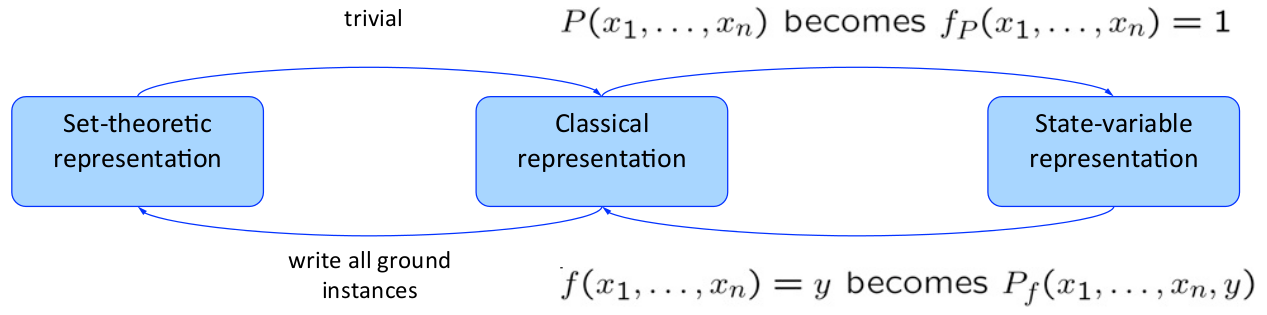
\includegraphics[width=0.48\textwidth]{./img/conversions.png}

\end{itemize}